\documentclass[journal]{IEEEtran}
\usepackage{amsmath,amssymb,amsfonts}
\usepackage{booktabs}
\usepackage{graphicx}
\usepackage{xcolor}
\usepackage{algorithm}
\usepackage{algorithmic}
\usepackage[hidelinks]{hyperref}

\newcommand{\method}{RAAR}
\newcommand{\methodlong}{Rubric-Anchored Adversarial Refinement}
\newcommand{\bench}{LvUP-Bench}
\newcommand{\opus}{Claude Opus 4.8}
\newcommand{\fable}{Claude Fable 5}
\newcommand{\gptjudge}{GPT-5.5 judge}

\begin{document}

\title{Inference-Time Scaffolding Across Two Axes: Closing a
Cross-Generation Gap and Climbing a Model-Tier Ladder with
Rubric-Anchored Adversarial Refinement}

\author{Jinbae~Park%
\thanks{J. Park is an independent researcher (e-mail: jinbae@pyne.work).}%
\thanks{Code, benchmark, checkers, and raw experimental artifacts are available
at \url{https://github.com/bubilife1202/Model_LvUP}.}}

\markboth{Preprint, June 2026}{Park: Inference-Time Scaffolding Across Two Axes}

\maketitle

\begin{abstract}
Frontier language-model upgrades matter along two practical axes: a direct
successor can replace an older flagship, and a cheaper tier can displace a
frontier tier if better inference-time scaffolding recovers enough quality.
We study both with \methodlong{} (\method{}), a five-stage loop that fixes a
binary success rubric before generation, diversifies candidates, verifies
each adversarially in a fresh context, fuses verified strengths, and exits
when a fresh verifier fails to refute the answer or a bounded revision
budget is spent. Study~1 compares
\opus{}+\method{} against \fable{} single-pass on \bench{} v1. The measured
objective gap concentrates in one precision-writing task; there \method{}
recovers 5 of the 7 constraint checks the predecessor misses (71\%,
$n{=}4$), lifting the macro-average from 0.971 to 0.992 against the
successor's 1.000, with no loop run scoring below the base model in 14
runs. Study~2 introduces \bench{} v2, a headroom-seeking ladder benchmark
with 12 objective tasks and 3 judged tasks; one constrained writing item is
excluded from primary analysis because collection failed and left an
incomplete no-answer cell. Post-hoc, Fable remains near ceiling on most scored
objective tasks, so frontier-gap claims use an explicit Fable-over-base
headroom filter. On the 5 common verification-shaped tasks where Sonnet
trails Fable by more than 0.05 under that documented rule,
Sonnet+\method{} closes 0.733 of the filtered gap
(95\% CI $[0.300, 1.067]$, $n{=}5$); this headline is threshold-sensitive
(0.50--0.73 as the tiny-denominator headroom cutoff moves from 0.02 to 0.10,
and 0.42 pooled across all 10 tasks), and across all 10 common scored tasks
Sonnet+\method{} remains 0.137 below Fable single-pass ($p{=}0.127$). Haiku+\method{} gains
0.274 absolute on 11 matched primary tasks but closes only 0.304 of its
Fable gap (95\% CI $[-0.111, 0.639]$). At Sonnet tier, Self-Refine is numerically the
strongest loop arm, and on the matched 11-task primary set the loop family
lifts Sonnet base from 0.730 to 0.820--0.901 (the upper value is
Self-Refine on the same 11-task denominator; its scored-available 12-task
macro is 0.873) with no measurable separation among loop variants.
A direct-answer Sonnet control
falls to 0.478, consistent with deliberation being load-bearing. Across
the two studies, the practical reading is bounded but useful: one tier down
plus \method{} can narrow the gap toward \emph{unscaffolded} frontier output
(Fable single-pass) on a filtered verification-shaped subset --- we did not complete
an equal-scaffolding (Fable+\method{}) frontier control --- whereas
open-ended coherence tasks and two-tier drops do not recover.
\end{abstract}

\begin{IEEEkeywords}
Large language models, test-time compute, inference scaling, self-refinement,
LLM-as-a-judge, verification.
\end{IEEEkeywords}

\section{Introduction}
\IEEEPARstart{F}{rontier} language models now improve along two practical
axes at once. A direct successor replaces an older flagship; below that,
cheaper serving tiers shadow the frontier closely enough that a better
calling pattern may be more attractive than a weight switch. Both cases
raise the same engineering question: how much of the quality difference is
\emph{recoverable at inference time}, by spending more compute through a
better scaffold rather than by changing the model? The question matters
wherever model swaps are slow or impossible --- regulated deployments pinned
to audited versions, cost-tiered products, and the long tail of systems
that cannot re-validate against every new release. It is also a clean
scientific probe: inside one vendor family, gap closure isolates capability
progress from the vendor- and data-confounds that plague cross-family
comparisons.

The test-time-compute literature gives a partial answer. With a reliable
external verifier, inference compute substitutes for parameters: a
compute-optimally sampled small model can outperform a $14\times$ larger one
on MATH \cite{snell2024}, repeated sampling lifts an inexpensive open code
model from 15.9\% to 56\% coverage on SWE-bench Lite \cite{brown2024}, and a
trained verifier is worth a $30\times$ parameter increase on GSM8K
\cite{cobbe2021}. But these results live where ground truth is checkable.
The negative results live everywhere else: without external feedback,
intrinsic self-correction \emph{degrades} reasoning \cite{huang2023}, GPT-4
self-critique collapses on planning tasks \cite{stechly2024}, self-refinement
stalls once the model is confident \cite{liang2023}, and models
systematically prefer their own generations \cite{panickssery2024,
wataoka2024}. Worse, the self-improvement gap saturates within a few
iterations \cite{song2024}, and imperfect verifiers impose accuracy ceilings
that no resampling budget breaks \cite{stroebl2024}.

This paper studies both axes with one loop, \methodlong{} (\method{}).
Study~1 revisits the hardest same-family question: can an older flagship,
\opus{}, recover a direct successor, \fable{}, at inference time?
Study~2 asks the deployment question practitioners often face first: how
far up a model-tier ladder can the same loop lift cheaper tiers on a
benchmark with calibrated headroom? \method{} uses the model's own weights
in five role-separated, fresh-context stages: rubric externalization before
any solution exists, strategy-diversified parallel generation,
evidence-quoting adversarial verification, defect-aware fusion, and a
\emph{burden-of-proof-flipped exit gate} that terminates only when a fresh
adversarial verifier fails to refute the candidate. The design is
deliberately conservative about every published failure mode: no role ever
critiques inside the context that generated the artifact (defusing
self-preference, whose mechanism is self-recognition
\cite{panickssery2024}), critique is anchored to externally fixed binary
rubrics (converting unreliable holistic judgment into reliable per-item
checks \cite{tick2024, rar2025}), and revision rounds are capped at the
saturation horizon the self-improvement literature predicts \cite{song2024}.

The two studies land in different but compatible places. On \bench{} v1,
the objective generation gap between \opus{} and \fable{} concentrates in
a single precision-writing task, and there \method{} recovers 5 of the 7
constraint checks the predecessor misses ($71\%$, $n{=}4$), lifting the
macro-average from 0.971 to 0.992 against the successor's 1.000, with no
loop run scoring below the base model in any of 14 runs. On \bench{} v2,
the overall Sonnet lift is modest on 11 matched primary objective tasks
($+0.089$, $p{=}0.521$), but the task-conditional story is sharper:
Sonnet+\method{} closes about 73\% (threshold-sensitive: 0.50--0.73,
or 0.42 pooled) of the filtered Fable gap on the 5 common tasks where
Fable's headroom over Sonnet exceeds 0.05 (95\% CI $[0.300, 1.067]$, $n{=}5$), while Haiku+\method{} improves in absolute
score ($+0.274$, $p{=}0.042$) yet recovers only 0.304 of its gap (95\% CI
$[-0.111, 0.639]$). At Sonnet tier, Self-Refine reaches the best
scored-available macro (0.873 over 12 task means) and, on the matched
11-task primary set, the loop family lifts base Sonnet from 0.730 to
0.820--0.901 without a measurable separation among loop variants. Together
the studies say that
iteration alone is not the active ingredient; the recoverable part of the
gap is task-shaped, tier-shaped, and mediated by
\emph{adversarially gated, rubric-anchored, context-decoupled}
deliberation.

A scope clarification is important for interpreting the released artifact.
The generator comparisons in this version are Claude-family comparisons:
\opus{}, Sonnet, Haiku, and \fable{}. GPT-5.5 appears only in the blinded
judging pipeline. The artifact does not contain a GPT-5.5 generation arm, so
this paper does not claim that \method{} has been measured on GPT-5.5 as a
generator.

Concretely, the paper does four things. It defines \method{} as a
role-separated, rubric-anchored inference scaffold; builds two small
benchmark regimes with mechanical checkers and blinded judged tails; collects
Claude-family generator outputs under single-pass, looped, and ablation arms;
and reports the resulting wins, failures, missing cells, and adversarial audit
findings in one inspectable artifact. The goal is not a leaderboard claim.
The goal is to make the boundary visible: where call structure appears to
recover a model-tier gap, where it fails, and what future controls would be
needed for a stronger claim.

Our contributions:
\begin{itemize}
\item \textbf{\method{}}, an inference-time loop whose every component is
motivated by a documented failure mode of naive refinement, and whose key
novelty --- a generated instance-specific rubric acting as a synthetic weak
verifier that \emph{gates loop exit} on otherwise unverifiable tasks ---
extends verifier-gated test-time compute beyond math and code
(Section~\ref{sec:method}).
\item \textbf{Two benchmark regimes under one artifact:} \bench{} v1, a
small contamination-controlled cross-generation benchmark, and
\bench{} v2, a headroom-seeking ladder benchmark with 12 objective
tasks and 3 judged tasks, transparent failed cells, one disclosed
task exclusion from primary analysis due to failed no-answer collection,
and an explicit post-hoc saturation caveat for frontier-tier
cells (Sections~\ref{sec:bench} and~\ref{sec:study2}).
\item \textbf{A two-study empirical answer:} Study~1 evaluates
predecessor + loop vs.\ direct successor; Study~2 evaluates the same loop
across cheaper model tiers, with explicit permutation tests for all
significance claims and a cross-family judged panel for open-ended tasks
(Sections~\ref{sec:results} and~\ref{sec:study2}).
\item \textbf{A practical playbook, not just a win/loss headline:}
\method{} helps most on verification-shaped tasks with remaining headroom,
can narrow a one-tier-down model's gap to unscaffolded frontier output on the
measured headroom slice, does not clearly recover two-tier drops, and remains weak on
coherence-shaped prose (Section~\ref{sec:study2-domain}).
\item \textbf{A diagnostic artifact for follow-on work:} the release keeps raw
outputs, sanitized Study~1 role-separated message transcripts, scored rows,
failed/no-answer cells, judge manifests, checker hardening notes, and
adversarial-review findings together so that later work can reproduce,
criticize, extend, or falsify the boundary map rather than trust a compressed
headline.
\end{itemize}

\section{Related Work}
\textbf{Test-time compute scaling.} Snell et al.~\cite{snell2024} showed
compute-optimal inference scaling can beat a $14\times$ larger model
FLOPs-matched; Brown et al.~\cite{brown2024} established log-linear coverage
growth under repeated sampling; Liu et al.~\cite{liu2025} pushed a 1B model
past a 405B model on MATH-500 with process-reward-guided search; s1
\cite{s1_2025} reproduced o1-style scaling with budget forcing. The
consistent precondition is a \emph{verifier}: Setlur et
al.~\cite{setlur2025} prove verifier-free test-time scaling is suboptimal by
a $\sqrt{H}$ factor, and every weak-beats-strong result above relies on
automatic checking. Conversely the limits are documented: best-of-$n$
degrades past $n\!\approx\!400$ through verifier hacking \cite{cobbe2021},
false-positive verifiers impose hard ceilings \cite{stroebl2024}, and longer
deliberation can \emph{hurt} via distractor amplification
\cite{gema2025}. \method{} inherits the verifier-gated paradigm but
\emph{manufactures} the verifier --- an instance-specific rubric generated
before any candidate exists --- so the paradigm applies to unverifiable
tasks, and caps all iteration far below the hacking and saturation regimes.
The closest prior comparisons are same-family but cross-\emph{scale}:
Liu et al.~\cite{liu2025} pit a 1B Llama against a 405B sibling using
trained process reward models on math; Snell et al.'s comparisons are
likewise intra-family with external verifiers on verifiable tasks. Our
setting differs on the three axes that matter for the deployment question:
frontier predecessor vs.\ \emph{direct successor} at comparable scale, no
trained or programmatic verifier available to the loop, and open-ended
tasks among the targets.

\textbf{Self-refinement and its failure modes.} Self-Refine
\cite{madaan2023} and Reflexion \cite{shinn2023} popularized
iterative self-feedback. Subsequent negative results sharpened the picture:
intrinsic self-correction without external signals degrades reasoning
\cite{huang2023}; self-verification collapses on planning
\cite{stechly2024}; refinement stalls at confident wrong answers
\cite{liang2023}; the generator--validator gap means the internal judge
agrees with the internal generator only 76\% of the time even for GPT-4
\cite{li2023gv}; and self-improvement capacity saturates in a few rounds
with collapsing diversity \cite{song2024, huang2024sharpening}. \method{}
treats this literature as a design specification (Section~\ref{sec:principles}).

\textbf{Multi-candidate generation and fusion.} Self-consistency
\cite{wang2022} and LLM-Blender \cite{jiang2023} established that sampling
plus rank-or-fuse beats single passes; Mixture-of-Agents \cite{wang2024moa}
beat GPT-4o with open models, while Self-MoA \cite{selfmoa2025} showed
single-model sampling diversity often suffices --- convenient for our
single-model setting. Debate-style multi-agent setups help factuality
\cite{du2023} but do not reliably beat self-consistency at matched cost
\cite{smit2024}; we therefore use directive-diversified parallel generation
rather than inter-agent dialogue, and fuse with defect evidence instead of
ranking alone.

\textbf{Rubrics and checklists.} Instance-specific binary checklists
materially improve both evaluation agreement and downstream refinement
(TICK/STICK \cite{tick2024}; CheckEval \cite{checkeval2024}); rubric-based
rewards yield the largest gains for the \emph{weakest} judges
\cite{rar2025}, which is exactly the property a predecessor-model verifier
needs; rubric scaffolds also steer generation when shown up front
\cite{ruscarl2025}. Prior work scores or trains with rubrics; \method{} is,
to our knowledge, the first to let a self-generated rubric \emph{gate loop
termination} at inference time.

\textbf{Judging hygiene.} LLM judges suffer position bias strong enough to
flip rankings \cite{wangfair2023}, verbosity bias \cite{zheng2023}, and
self-preference driven by self-recognition \cite{panickssery2024,
wataoka2024}. Our evaluation therefore scores objective tasks purely
mechanically, and judged tasks with position-swapped pairwise comparisons
across three model families, so no family's self-preference decides any
comparison involving its own output.

\textbf{Scaffolding as a capability lever.} On agentic benchmarks,
interface and scaffold design alone moves a fixed model by a factor of
three \cite{yang2024sweagent}, simple scaffolds rival agentic ones
\cite{xia2024agentless}, and deliberate ensembles of weak verifiers
approach frontier-model accuracy \cite{saadfalcon2025}.
\method{} is the pure-text analog: no tools, no retrieval, no environment
--- the entire lever is call structure.

\section{The \method{} Loop}
\label{sec:method}

\subsection{Setting and Notation}
Let $M_w$ denote a \emph{base} model (here \opus) and $M_s$ a \emph{target}
model (here \fable), where $M_s$ dominates $M_w$ in single-pass output quality
on a task distribution $\mathcal{T}$. Given a task $x \in \mathcal{T}$, a
single-pass arm produces $y = M(x)$ with one inference call. An
\emph{inference-time scaffold} $S$ produces $y = S^{M_w}(x)$ using only calls
to $M_w$ --- the same weights in every role --- and no external information.
The question we study is whether a scaffold can close the \emph{generation
gap} $\Delta(x) = q(M_s(x)) - q(M_w(x))$, where $q$ is task quality measured
by an oracle (hidden tests, exact answers, mechanical checkers) or by a blind
cross-family judge panel.

\subsection{Design Principles}
\label{sec:principles}
\method{} is built from three observations, each grounded in prior failure
analyses of naive refinement loops:

\textbf{P1 --- Verification is easier than generation.} For the task families
we study, checking a candidate against an explicit criterion (recomputing an
arithmetic step, tracing code on a boundary input, counting sentences)
requires strictly less capability than producing a flawless artifact in one
pass. A model too weak to generate $M_s$-grade output in one call can still
be a reliable \emph{detector} of the defects that separate its output from
$M_s$'s.

\textbf{P2 --- Self-evaluation in-context is corrupted by self-consistency.}
When the same context that produced an answer is asked to critique it, the
critique inherits the generation's blind spots and exhibits sycophantic
self-approval; this is the documented failure mode of intrinsic
self-correction. The fix is structural, not exhortative: every evaluative
role in \method{} runs in a \emph{fresh context} that never sees the
reasoning that produced the artifact under review, and is told the artifact
was written by someone else.

\textbf{P3 --- Exit conditions must flip the burden of proof.} A loop that
exits when a critic \emph{approves} converges to whatever the critic is too
lazy to object to. \method{} exits only when an adversarial verifier,
explicitly mandated to hunt for defects with per-criterion evidence,
\emph{fails to refute} the answer. Approval is the absence of surviving
objections, not the presence of praise.

\subsection{The Five Stages}
\label{sec:stages}
Algorithm~\ref{alg:raar} gives the full loop; all five roles are played by
$M_w$ in stateless, fresh-context calls.

\textbf{Stage 1: Rubric externalization.} Before any solution attempt, a
fresh instance is asked to produce 8--12 \emph{binary, mechanically
checkable} success criteria for the task: correctness requirements, exact
output-format requirements, and the typical failure modes of the task
family. The rubric instance is forbidden from solving the task, so that
the rubric does not inherit a particular solution's blind spots --- an
instruction, not a guarantee: Section~\ref{sec:rubric-case} documents one
run in which the rubric violated it and the loop survived anyway. The
rubric then
anchors every downstream role: generators see it as the grading contract,
verifiers check against it criterion by criterion, and the fuser uses it to
arbitrate between candidates. This converts the vague instruction
``be correct'' into a concrete, shared checklist --- the loop's fixed point
is defined \emph{before} the first candidate exists.

\textbf{Stage 2: Diversified generation.} $K{=}3$ generators run in
parallel, each with the task, the rubric, and a distinct strategy directive
(decompose-first; enumerate-typical-failures-first; direct-expert-pass with
line-by-line re-verification). Distinct directives decorrelate failure
modes: the candidates fail in different places, which is what makes
cross-candidate fusion (Stage 4) informative.

\textbf{Stage 3: Adversarial verification.} Each candidate is reviewed by a
fresh verifier instance that (i) is told the answer ``was written by someone
else and likely contains defects,'' (ii) must walk \emph{every} rubric
criterion quoting evidence, (iii) must independently recompute any
computation rather than trusting it, and (iv) must grade each defect FATAL /
MAJOR / MINOR. The mandate to hunt --- with per-criterion evidence
obligations --- is what defeats the rubber-stamp equilibrium.

\textbf{Stage 4: Fusion.} A fresh instance receives all $K$ candidates
\emph{with their defect reports} and composes a single answer: start from
the strongest candidate, graft superior fragments from the others, fix every
flagged defect (re-verifying each flag, since verifiers can be wrong).
Fusion-with-evidence is strictly stronger than best-of-$K$ selection: it can
repair the best candidate's verified defects with material from candidates
that got those parts right.

\textbf{Stage 5: Burden-flipped gate.} A fresh adversarial verifier reviews
the fused answer under the same mandate. If it reports any FATAL or MAJOR
defect, the defect report is handed to a fresh revision instance
(which never sees the fuser's reasoning, only its artifact), and the gate
repeats; the loop exits when the verifier fails to refute, or after $R{=}2$
revisions. Note the asymmetry of the second exit: a cap-exhausted run
returns its final revision \emph{unverified}; Section~\ref{sec:gate-analysis}
reports how often this happened and what it cost.

\begin{algorithm}[t]
\caption{\method{}: \methodlong{}}
\label{alg:raar}
\begin{algorithmic}[1]
\REQUIRE task $x$, base model $M_w$, $K{=}3$, $R{=}2$
\STATE $\rho \leftarrow M_w(\textsc{Rubric}(x))$ \hfill$\triangleright$ no solving allowed
\FOR{$i = 1 \dots K$ \textbf{in parallel}}
  \STATE $c_i \leftarrow M_w(\textsc{Gen}(x, \rho, d_i))$ \hfill$\triangleright$ directive $d_i$
\ENDFOR
\FOR{$i = 1 \dots K$ \textbf{in parallel}}
  \STATE $v_i \leftarrow M_w(\textsc{Verify}(x, \rho, c_i))$ \hfill$\triangleright$ fresh context
\ENDFOR
\STATE $y \leftarrow M_w(\textsc{Fuse}(x, \rho, c_{1..K}, v_{1..K}))$
\FOR{$r = 1 \dots R$}
  \STATE $g \leftarrow M_w(\textsc{Verify}(x, \rho, y))$
  \IF{$g$ reports no FATAL/MAJOR defect} \STATE \textbf{break} \ENDIF
  \STATE $y \leftarrow M_w(\textsc{Revise}(x, \rho, y, g))$
\ENDFOR
\RETURN $y$
\end{algorithmic}
\end{algorithm}

\subsection{Why the Gate is the Kick}
\label{sec:kick}
Each stage of \method{} has published precedent except the one that does the
disproportionate work: the combination, in Stages 3 and 5, of
\emph{rubric-anchored adversarial verification} with a
\emph{burden-of-proof-flipped exit}. We call this the loop's kick, and the
mechanism is worth stating precisely.

A single-pass generation by $M_w$ fails not because $M_w$ lacks the
knowledge to avoid its mistakes, but because generation must get every
decision right \emph{jointly} in one sampled trajectory, while the model's
reliability per decision is below the threshold that the conjunction
requires. Verification decomposes the conjunction: each rubric criterion is
checked \emph{independently}, in a fresh context, with no commitment to any
prior trajectory. As a motivating heuristic --- not a validated mechanism
--- if $M_w$ detects a defect of the relevant class with probability $d$
per inspection, and inspections are roughly decorrelated across fresh
contexts, the probability that a defect survives the candidate-stage
review plus $R$ gate reviews falls like $(1-d)^{R+1}$, while a single-pass
generation gets exactly one chance to avoid introducing it. Both
assumptions can fail: detection rates are defect-class-dependent, and the
shared rubric correlates inspections across rounds --- our T4 counting
residue and the rubric-poisoning run of Section~\ref{sec:rubric-case} are
exactly such failures, and we report them as the method's boundary. The
heuristic's core survives the caveats: the loop converts a
\emph{per-trajectory} reliability problem into a \emph{per-criterion}
detection problem, and detection is the easier side of the
generator--verifier asymmetry \cite{cobbe2021, setlur2025, weiblog2025}.

Three structural choices keep this argument from collapsing in practice,
each neutralizing a documented failure mode:

\emph{(i) The rubric exists before any candidate.} A critic asked ``is this
good?'' free-associates criteria correlated with the answer's own framing
--- the generator--validator inconsistency of \cite{li2023gv}. Fixing 8--12
binary criteria from the task statement alone makes the verification target
exogenous to every candidate, so a candidate cannot look correct merely by
defining the terms of its own grading. This is why rubric quality gains are
largest for weak judges \cite{rar2025}: the rubric carries the judgment
structure the judge would otherwise have to improvise.

\emph{(ii) The verifier is adversarial by mandate, with evidence
obligations.} Free-running critics rubber-stamp once the artifact looks
fluent --- the confidence stall of \cite{liang2023} and the self-approval
documented by \cite{huang2023}. \method{}'s verifier is told the artifact
was written by someone else (attacking the self-recognition channel of
self-preference \cite{panickssery2024}), is required to walk every
criterion quoting evidence, and is required to recompute any computation it
encounters. It may conclude PASS only as a \emph{failure of an active
refutation attempt}, never as an impression.

\emph{(iii) The exit condition is refutation-failure, not approval.} A loop
that exits on approval optimizes for whatever makes critics approve ---
Goodhart pressure toward confident-sounding output. A loop that exits only
when a fresh adversary finds nothing FATAL or MAJOR optimizes for
\emph{indefensibility of objections}, which is the actual quality target.
The asymmetry matters: approval is one bit produced cheaply; a failed hunt
is a costly certificate that correlates with genuine absence of detectable
defects. Because gap saturation bounds how many rounds can help
\cite{song2024}, the gate is capped at $R{=}2$ revisions --- the certificate
is bought at bounded cost.

The ablations in Section~\ref{sec:results} make the attribution concrete:
best-of-3 shares \method{}'s diversity but not its verification and gains
little; Self-Refine shares its iteration but not its role separation or
rubric anchor and gains less, exactly as the negative-results literature
predicts \cite{huang2023, stechly2024}.

\section{Study 1: Cross-Generation Gap on \bench{} v1}
\label{sec:results}
\label{sec:study1}

\subsection{\bench{} v1 and Setup}
\label{sec:bench}
\label{sec:setup}
Study~1 is the original cross-generation experiment in this paper, now
reframed as the first half of a two-study argument. Comparing scaffolds
across \emph{models} requires unusual care: public benchmark items may sit
in either model's training set, and judge models prefer their own family's
prose. \bench{} v1 controls both.

\textbf{Objective core (5 tasks).} (i)~\emph{T1 interval algebra}: implement
an \texttt{IntervalSet} class with open/closed endpoint semantics, set
difference (\texttt{remove}) with closedness flips at cut points, point
intervals, and canonical string output; graded by 40 hidden tests covering
endpoint-merge and removal case analysis. (ii)~\emph{T2 seeded bug-fix}: a
sliding-window rate limiter with four seeded boundary/recording bugs and an
authoritative prose spec; graded by 10 hidden tests constructed so that
partial fixes are caught (one seeded bug masks two others, so only the
complete fix passes). (iii--iv)~\emph{T3 combinatorics} ($\times 2$): novel
counting problems whose answers (293{,}749 and 324{,}288) were computed by
two independent programs that agree; graded by exact match.
(v)~\emph{T4 constrained writing}: a paragraph that must satisfy 12
simultaneous mechanical constraints; graded by a deterministic checker,
score = fraction of constraints met. All objective items were constructed
for this study and mechanically verified.

\textbf{Semi-objective and judged tail.} \emph{T5 code review} is a 60-line
database service module with six seeded defects, scored by seeded-defect
recall. \emph{T6} (multi-region rate-limiter design document) and
\emph{T7} (WAL/fsync durability explanation) are open-ended and scored by
blind pairwise comparison with position swap from a four-judge,
three-family panel: \gptjudge{}, Gemini, \fable{}, and \opus{}. GPT-5.5 is
used here only as a judge, not as a generation arm. No
family holds a panel majority, and the two Claude judges never disagreed
with the cross-family majority in any cell.

\textbf{Arms and execution.} The arms are \opus{} single-pass;
\method{}$^{\text{Opus 4.8}}$; \fable{} single-pass; Self-Refine on
\opus{} with two feedback--refine rounds (5 calls); and best-of-3 on
\opus{} with an LLM selector (4 calls). All arms ran on 12 June 2026
against \texttt{claude-opus-4-8} and \texttt{claude-fable-5} with
vendor-default settings via Claude Code subagent calls. Objective code
tasks used 2 independent runs per arm, math tasks 3, the constraint task
4, and judged tasks 1 run per arm. Single-pass arms make 1 call;
Self-Refine 5; best-of-3 4; \method{} 9--12 depending on gate outcomes
(mean 10.5 over all runs).

\textbf{Model and tool disclosure.} Experimental generation is limited to
the model labels recorded in the released run artifacts. Study~1 generation
used \texttt{claude-opus-4-8} and \texttt{claude-fable-5}; Study~2 generator
rows in \texttt{results/v2/all\_runs.scored.json} are labeled
\texttt{haiku}, \texttt{sonnet}, \texttt{opus}, and \texttt{fable}. No
GPT-5.5 output is used as a scored generated answer. GPT-5.5 and
Gemini-family tools are used as blinded pairwise judges in the released
judging artifacts, alongside \texttt{claude-fable} and
\texttt{claude-opus} judges in Study~1. The manuscript, code, benchmark,
and checks were developed with AI-assisted drafting, coding,
debugging, checking, and adversarial review; the author reviewed the artifacts
and is responsible for all claims, data, code, and citations.

\subsection{Objective Tasks}
\label{sec:objective-results}
Table~\ref{tab:objective} and Fig.~\ref{fig:scores} give per-task mean
scores; Fig.~\ref{fig:macro} the macro-average.

\begin{table}[t]
\caption{Objective-task scores (mean over runs; 1.0 = all hidden tests /
constraints / exact answers correct). $n$ per cell: T1, T2 $=2$; T3a, T3b
$=3$; T4 $=4$.}
\label{tab:objective}
\centering
\small
\setlength{\tabcolsep}{2.3pt}
\begin{tabular}{lccccc}
\toprule
 & \multicolumn{4}{c}{Opus 4.8} & Fable 5 \\
\cmidrule(lr){2-5}
task & single & +SR & +Bo3 & +\method{} & single \\
\midrule
T1 interval code & 1.000 & 1.000 & 1.000 & 1.000 & 1.000 \\
T2 seeded bugfix & 1.000 & 1.000 & 1.000 & 1.000 & 1.000 \\
T3a combinatorics & 1.000 & \textbf{0.000} & 1.000 & 1.000 & 1.000 \\
T3b combinatorics & 1.000 & 1.000 & 1.000 & 1.000 & 1.000 \\
T4 constraints & 0.854 & 0.979 & 0.854 & 0.958 & 1.000 \\
\midrule
macro-average & 0.971 & 0.796 & 0.971 & \textbf{0.992} & 1.000 \\
\bottomrule
\end{tabular}
\end{table}

\begin{figure}[t]
\centering
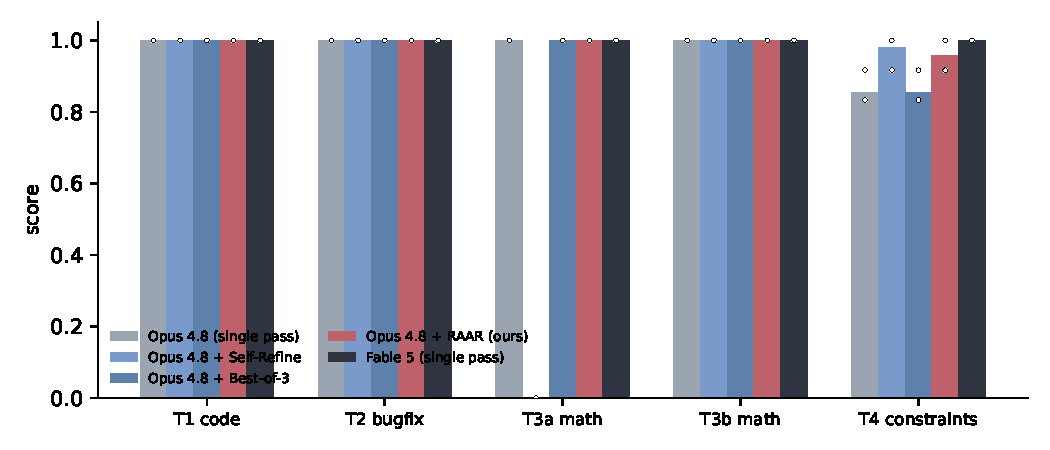
\includegraphics[width=\columnwidth]{fig_scores.pdf}
\caption{Per-task scores; dots are individual runs.}
\label{fig:scores}
\end{figure}

\begin{figure}[t]
\centering
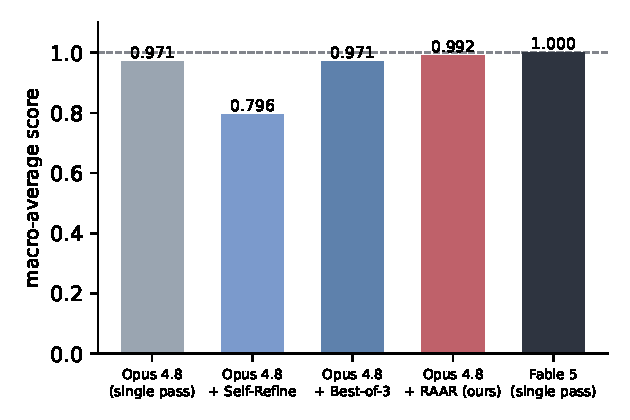
\includegraphics[width=0.9\columnwidth]{fig_macro.pdf}
\caption{Macro-average over the five objective tasks. The dashed line is the
Fable 5 single-pass target.}
\label{fig:macro}
\end{figure}

Three findings.

\textbf{(1) The objective generation gap is narrow and concentrated.} On
four of five objective tasks, \opus{} single-pass already matches \fable{}
at ceiling --- code synthesis with adversarial edge cases, seeded bug
fixing, and both novel combinatorics problems no longer separate these
generations at this difficulty. The entire measured objective gap lives in
T4, the 12-constraint precision-writing task, where \fable{} is exact
(12/12 on all 4 runs) and \opus{} reliably miscounts.
The failures are all \emph{exact-counting} constraints --- the sentence
count, the total and first-sentence word counts, and the
exactly-one-exclamation requirement (C1--C3, C8); the non-counting
constraints (keyword frequencies, positional and length caps) hold. This
specificity is itself a contribution of the contamination-controlled
design: with novel, mechanically scored items, ``the successor is better''
reduces to a specific, measurable competence --- exact composition under
simultaneous counting constraints --- rather than a diffuse impression.

\textbf{(2) \method{} closes most of the gap that exists and opened no new
one in any observed run.} On T4, \method{} lifts \opus{} from 0.854 to
0.958, recovering 5 of the 7 constraint checks the base arm missed
($71\%$, $n{=}4$ runs per arm with scores quantized in twelfths); on the
macro-average it reaches 0.992 vs.\ \fable{}'s 1.000. The single-task
provenance matters: T4 is the only objective task with headroom, so the
macro-average movement \emph{is} the T4 movement, and at this $n$ the
difference between \method{} (0.958) and Self-Refine (0.979) on T4 is not
separable from noise --- the cross-task pattern, not any one cell, is the
evidence. Equally important is the \emph{no-harm} observation: across all
14 \method{} runs, not one scored below the \opus{} single-pass mean on
its task (an all-of-14 observation, compatible at 95\% confidence with a
true per-run harm rate as high as $\sim$20\%). The loop's gate refused 8
of 14 first-round fused answers (Section~\ref{sec:gate-analysis}), and no
run that passed through revisions ended below its task's base mean.

\textbf{(3) Iteration without structure is actively destructive ---
replicating the negative literature.} Self-Refine \emph{destroyed} T3a: the
base model answers 293{,}749 correctly in 3 of 3 single passes, but after
two self-feedback rounds the final answers were 293{,}589, 220{,}815, and
293{,}875 --- three different corruptions, scoring 0/3. The trajectory
transcripts (shipped in the artifact) confirm at least one chain entered
refinement with the correct answer and was talked out of it by its own
critique (Section~\ref{sec:selfrefine-case}), the precise failure mode
documented by Huang et al.~\cite{huang2023} and the sharpening literature
\cite{song2024}. The same iteration budget inside \method{}'s structure
(fresh-context adversarial verification, evidence-gated revision) caused
zero such corruptions in 14 runs. Best-of-3, sharing \method{}'s sampling
diversity but not its verification, tracked the baseline exactly (0.971) ---
diversity alone neither helps nor hurts here.

\subsection{Semi-Objective: Seeded Code Review (T5)}
All five arms recalled all six seeded defects (6/6) --- defect-finding
recall at this density does not separate these models either. One
qualitative asymmetry survives: the module contains a genuine defect we did
not plant (a negative-quantity order credits the buyer's account). \fable{}
and every augmented \opus{} arm (Self-Refine, best-of-3, \method{})
surfaced it; \opus{} single-pass alone did not. Consistent with the
objective results, added inference structure recovered a successor-level
finding that the bare predecessor pass missed, though with $n{=}1$ this is
an observation, not a statistic.

\subsection{Judged Open-Ended Tasks}
\label{sec:judged-results}
Table~\ref{tab:judged} reports blind, position-swapped pairwise verdicts
from the four judges (\gptjudge{}, Gemini, \fable{}, \opus{}; 8 verdicts
per pair). Because the two orders are judged by the same judges, verdicts
within a cell are correlated; we therefore report exact counts and
unanimity rather than significance tests.

\begin{table}[t]
\caption{Blind pairwise judgments (wins out of 8; 4 judges $\times$ 2
position-swapped orders). 4--4 indicates no detectable preference.}
\label{tab:judged}
\centering
\small
\setlength{\tabcolsep}{4pt}
\begin{tabular}{lcc}
\toprule
comparison & T6 design & T7 explain \\
\midrule
Opus 4.8 vs.\ Fable 5 & 0 -- 8 & 0 -- 8 \\
\method{} vs.\ Fable 5 & \textbf{4 -- 4} & 0 -- 8 \\
\method{} vs.\ Opus 4.8 & \textbf{8 -- 0} & 6 -- 2 \\
\method{} vs.\ Self-Refine & 4 -- 4 & 1 -- 7 \\
\bottomrule
\end{tabular}
\end{table}

\textbf{On the design task the panel can no longer distinguish the looped
predecessor from the successor.} \opus{} single-pass loses to \fable{}
0--8 --- every judge, both orders. \method{} beats its own base 8--0 with
the same unanimity. Against \fable{} the count is 4--4, and the
\emph{structure} of the split is the finding: every one of the four judges
voted for position A in both orders, so the verdicts became purely
order-determined. We read this as indistinguishability rather than
``parity'' in any stronger sense --- when the quality signal vanishes,
position bias is all that remains, and that is precisely what unanimous
position-following indicates. This is the configuration the kick predicts:
a design
document is a bundle of independently checkable commitments (algorithm
choice, partition behavior, capacity arithmetic, failure modes), exactly
the structure an externalized rubric and an evidence-quoting verifier can
grind through.

\textbf{On the explanation task the gap narrows but does not close.}
\method{} beats its base 6--2, but \fable{} still wins 8--0 against both
\opus{} arms. Notably, Self-Refine beats \method{} 7--1 here --- the one
setting in our study where unstructured polish outperforms structured
verification. The pattern is informative: T7 quality is dominated by
pedagogical coherence --- one running example sustained across a long
causal chain --- which a holistic rewrite preserves and fusion-of-three-%
candidates fragments. Together with T3a (where Self-Refine destroys
correctness that \method{} preserves), the two tasks bracket the design
space: \emph{verification-shaped tasks reward \method{}; coherence-shaped
tasks reward gentler iteration; and using the wrong loop for the task class
is not a small mistake in either direction.}

Two hygiene notes. First, output length: \method{} answers are the longest
in every judged cell (T6: 12.7k characters vs.\ \fable{}'s 9.2k and
\opus{}'s 8.5k; T7: 8.5k vs.\ 5.8k), so verbosity bias \cite{zheng2023}
plausibly assists \method{} in the cells it wins; we note, however, that
the two cells \method{} \emph{loses} unanimously (T7 vs.\ \fable{} and
vs.\ the shorter Self-Refine) go against the length gradient, so length
alone does not explain the pattern. Second, one judge verdict was unstable:
a duplicated GPT-5.5-judge run on one T7 \method{}-vs.-base comparison returned
opposite verdicts; we keep the first-run verdict (6--2; the alternative
resolution gives 7--1, favoring \method{} more). The dedup rule ---
first verdict per (comparison, judge) --- is fixed in the artifact.

Across both judged tasks, the predecessor single-pass takes 0 of 16
verdicts against the successor; with \method{} it takes 4 of 16, all on
T6, where the panel's preference signal disappears entirely.

\section{Study 2: The Model-Tier Ladder on \bench{} v2}
\label{sec:study2}

\subsection{\bench{} v2 Benchmark Design}
Study~1's objective core largely saturated: four of five v1 objective tasks
were already at ceiling for \opus{} single-pass. \bench{} v2 was built to
restore headroom for cheaper-tier comparisons. Its construction spec targets
frontier single-pass scores between 0.3 and 0.85, requires pure text
completion with deterministic scoring, authoritative prompts, novel
instances, reference solutions that score 1.0, graded near-miss checks, and
dual-computation for math ground truth. The resulting benchmark has 12
objective tasks and 3 judged tasks, but the post-hoc Fable results show that
the frontier target was only partially achieved: Fable base is at or near
ceiling on most scored objective tasks. We therefore use v2 for measured
cheaper-tier headroom and report frontier saturation as a limitation, not as
evidence of broad frontier discrimination.
The validator certifies structural reproducibility, not publishability by
itself: empirical difficulty, novelty, prompt ambiguity, and the semantic
meaning of partial-credit magnitudes still require audit.
The primary objective set is 11 tasks across code (4), spec compliance (2),
math (4), and seeded code review (1); the twelfth objective task,
\texttt{constrained\_writing\_16}, is reported transparently but excluded
from primary analysis because collection failed and left an incomplete
no-answer cell. In the released artifact that task leaves a partial cell only:
base@sonnet has one scored run at 0.625 and one failed run, while
base-direct@sonnet and both raar@sonnet runs are failed no-answer cells, so
the task does not support a fair paired comparison.

All v2 items are novel to this study. Code and spec-compliance tasks use
hidden tests or exact file transformation; math tasks use exact answers
verified by two independent programs; the code-review task uses seeded-defect
recall; and the judged tail consists of \emph{design\_pipeline},
\emph{explain\_raft}, and \emph{migration\_plan}. Collection is intentionally
transparent about incompleteness. In the released scored artifact, the
scored objective-row counts are base@sonnet $n{=}34$,
raar@sonnet $n{=}33$, selfrefine@sonnet $n{=}17$,
bo10@sonnet $n{=}16$, raar-norubric@sonnet $n{=}15$,
raar-approval@sonnet $n{=}15$, base-direct@sonnet $n{=}11$,
base@haiku $n{=}22$, raar@haiku $n{=}16$, base@fable $n{=}19$, and
raar@fable $n{=}6$. We drop the Opus v2 cells from analysis because that
batch is incomplete and the base point shows an unexplained anomaly.

For judged tasks, completed Sonnet-vs.-Sonnet comparisons contribute
$n{=}2$ generation pairs, while frontier comparisons contribute $n{=}1$
pair when only one frontier generation completed. Study~1's
four-judge panel established that the Claude-family judges never flipped
cross-family majorities, so v2 keeps only the cross-family pair
(\gptjudge{} and Gemini), still with position swap, yielding 4 judgments
per generation pair
and a simpler conflict profile.

\subsection{Model-Matrix Results}
Figure~\ref{fig:ladder} gives the scored-available ladder view, and
Fig.~\ref{fig:cost} the same cells against mean calls. On the observed
objective cells, the ladder rises from base@haiku (macro 0.376 over
$n{=}11$ scored task means from 22 scored rows) to base@sonnet (0.721
over $n{=}12$ from 34 rows), while base@fable reaches 0.972 over $n{=}10$
from 19 rows. The looped and ablated Sonnet/Haiku/frontier arms are
raar@haiku 0.650 ($n{=}11$ task means; 16 rows), raar@sonnet 0.820
($n{=}11$; 33 rows), selfrefine@sonnet 0.873 ($n{=}12$; 17 rows; 0.901 on
the same 11-task primary denominator used for the Sonnet-family comparison),
bo10@sonnet 0.794 ($n{=}11$; 16 rows), raar-norubric@sonnet 0.834
($n{=}11$; 15 rows), raar-approval@sonnet 0.841 ($n{=}11$; 15 rows), and
raar@fable 0.967 ($n{=}5$; 6 rows). The direct-answer Sonnet control
lands at 0.478 over 11 task means from 11 rows.

\begin{figure*}[t]
\centering
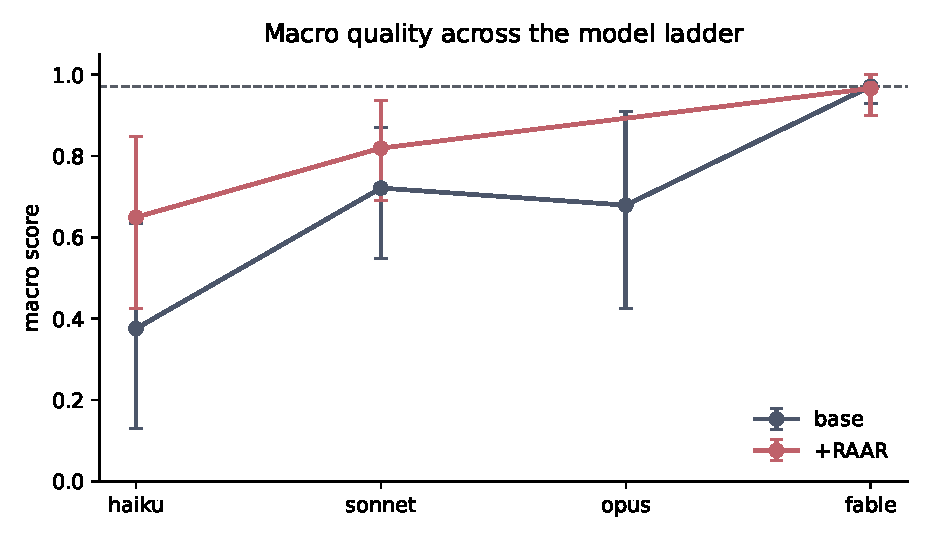
\includegraphics[width=0.88\textwidth]{fig_ladder.pdf}
\caption{Study~2 model ladder. Macros are computed over scored-available
objective task means. Primary inferential claims in the text use
common-task permutation tests and exclude
\texttt{constrained\_writing\_16}.}
\label{fig:ladder}
\end{figure*}

\begin{figure*}[t]
\centering
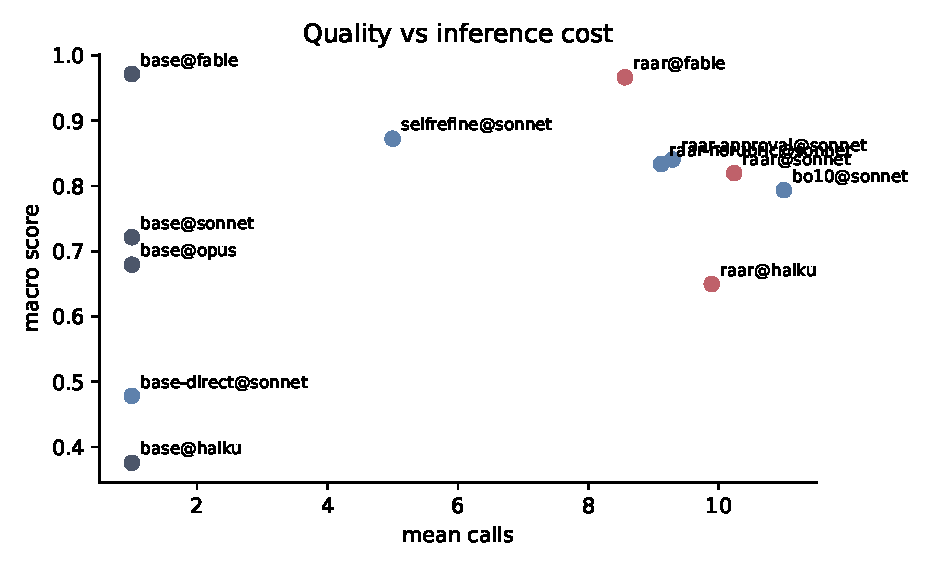
\includegraphics[width=0.88\textwidth]{fig_cost.pdf}
\caption{Study~2 quality vs.\ inference cost. Each point is a scored-available
objective cell; across all scored runs, Sonnet+\method{} averages 10.2
calls and Haiku+\method{} 9.9.}
\label{fig:cost}
\end{figure*}

The scored-available view is descriptive; the inferential claims come from
paired permutation tests on common tasks. On its full 11-task primary
objective set, Haiku+\method{} gains 0.274 over Haiku base ($n{=}11$,
$p{=}0.042$). Sonnet+\method{} gains 0.089 over Sonnet base ($n{=}11$,
$p{=}0.521$). Against Fable, however, the task-conditioned
picture is sharper than the overall macro. Gap closure is computed only on
tasks where Fable's single-pass advantage over the base model exceeds 0.05
(the headroom rule fixed in \texttt{stats.json}); smaller denominators make
the ratio unstable. Sonnet trails Fable by more than 0.05 on exactly 5 such
common primary tasks --- \emph{absorb\_expect}, \emph{csv\_normalize},
\emph{digit\_count}, \emph{interval\_sched}, and \emph{seq\_runs} --- and
Sonnet+\method{} closes 0.733 of that filtered gap (95\% CI
$[0.300, 1.067]$, $n{=}5$). This number is fragile: the $>$0.05 cutoff
excludes exactly \emph{code\_review\_12} (denominator 0.042, a tiny-denominator
ratio); at cutoff 0.0 or 0.02 closure falls to 0.500, at 0.10 it is 0.667,
and pooled at the macro level over all 10 common tasks it is 0.419. We report
the full sensitivity rather than a single point. Across all 10 common scored tasks,
Sonnet+\method{} still sits 0.137 below Fable single-pass ($n{=}10$,
$p{=}0.127$), so the point estimate still favors Fable even though the
filtered headroom slice now excludes zero.

The Haiku result is more limited. Haiku+\method{} does improve in absolute
score by 0.274 on the 11-task primary set, but its mean Fable-gap closure is
only 0.304 (95\% CI $[-0.111, 0.639]$, $n{=}9$ tasks under the same
$>$0.05-headroom rule). The practical message is
therefore asymmetric: one tier down can get close on the verification-shaped
slice; two tiers down does not recover reliably.

\subsection{Direct-Answer Control: Base-Direct vs.\ \method{}}
The Sonnet direct-answer control remains mechanistically informative even
though it no longer clears the 0.05 line. The base-direct ablation --- a
single-call answer-only control without the role-separated scaffold --- has
macro 0.478 on 11 primary task means and trails Sonnet+\method{} by 0.341 on
the 11 matched primary tasks ($p{=}0.061$). The conservative claim is
therefore directional rather than confirmatory: whatever the rest of the
Sonnet-tier ablations do, the multi-call scaffold is load-bearing in
magnitude. The loop does not merely wrap a better prompt around the same
direct answer; removing the staged generation, verification, and fusion
structure is strongly destructive in observed score.

\subsection{Sonnet-Tier Ablations}
Study~2 also asks whether the distinctive Study~1 ingredient --- the
rubric-anchored adversarial gate --- clearly survives at a more capable tier
and a different task mix. At this $n$, the answer is no. Relative to
Sonnet+\method{}, best-of-10 differs by $-0.026$ on 11 matched tasks
($p{=}0.928$), Self-Refine by $+0.081$ on 11 tasks ($p{=}0.444$),
approval-exit \method{} by $+0.027$ on 10 tasks ($p{=}0.812$), and
no-rubric \method{} by $+0.019$ on 10 tasks ($p{=}1.0$). With $n{=}2$--3
on the key Sonnet cells, Self-Refine is numerically the strongest Sonnet arm
at macro 0.873, but the family of looped variants is statistically
indistinguishable at this scale.

That negative result matters. Study~1's objective pattern and transcript
analysis pointed strongly at the gate as the loop's kick. Study~2 does
\emph{not} clearly replicate that advantage at Sonnet tier on these task
families. The shared Sonnet pattern is instead robustness: on the matched
11-task primary set, the loop family lifts base Sonnet from 0.730 to
0.820--0.901, i.e.\ about $+0.09$ to $+0.17$; the 0.901 endpoint is
Self-Refine on that matched denominator, while its scored-available macro is
0.873 over 12 task means. The measured differences between sensible
scaffolds compress into noise at this $n$. The honest reading is that the
gate story is strongest when the base model still has visible headroom and
the tasks are tightly verification-shaped.

\subsection{Judged Open-Ended Tasks}
\label{sec:study2-judged}
Table~\ref{tab:judged-v2} reports the judged tail. The judged artifact now
contains 14 completed generation pairs, i.e.\ 28 blinded position-swapped
comparisons evaluated by the two-family panel (\gptjudge{} and Gemini) for 56
total verdicts. Single-pair frontier comparisons contribute 4 judgments;
the Sonnet-vs.-Sonnet cells use two generation pairs for 8. We do not run
significance tests on these cells.

\begin{table}[t]
\caption{Study~2 judged outcomes. Each completed frontier cell is 4
judgments (2 judges $\times$ 2 answer orders); Sonnet-vs.-Sonnet cells use
two generation pairs for 8 judgments. ``--'' marks a missing cell.}
\label{tab:judged-v2}
\centering
\footnotesize
\setlength{\tabcolsep}{3pt}
\begin{tabular}{lccc}
\toprule
comparison & design & explain & migration \\
\midrule
Sonnet base vs.\ Fable base & 0 -- 4 & 0 -- 4 & 0 -- 4 \\
Fable +\method{} vs.\ Fable base & 3 -- 1 & -- & 4 -- 0 \\
Sonnet +\method{} vs.\ Fable base & 0 -- 4 & 0 -- 4 & 0 -- 4 \\
Sonnet +\method{} vs.\ Sonnet base & 6 -- 2 & 4 -- 4 & 7 -- 1 \\
\bottomrule
\end{tabular}
\end{table}

Fable base still sweeps Sonnet base 4--0 on all three judged tasks, and
Sonnet+\method{} still loses 0--4 to Fable on all three. In other words,
the open-ended gap is not closed even one tier down. Against its own base,
however, Sonnet+\method{} is sharply split by task family: it wins
\emph{design\_pipeline} 6--2, ties \emph{explain\_raft} 4--4, and wins
\emph{migration\_plan} 7--1. The new Fable+\method{} judged pairs are
descriptive only but directionally favorable: 3--1 on
\emph{design\_pipeline}, 4--0 on \emph{migration\_plan}, and no completed
\emph{explain\_raft} pair. The coherence boundary remains where Study~1
already suggested it would be: migration planning is rich in independently
checkable operational commitments, whereas the Raft explanation is a long
causal exposition whose quality depends on coherent pedagogical flow.

\subsection{Domain-Effectiveness Map}
\label{sec:study2-domain}
The numeric checker scores support the same task-shape story. Fig.~\ref{fig:domain}
visualizes the Sonnet category deltas, while the domain map in
Table~\ref{tab:domainmap} summarizes
\texttt{docs/DOMAIN\_MAP.md}; by construction it uses numeric checker scores
only, and buckets with no scored base/RAAR overlap are omitted. The table
shows the Haiku and Sonnet tiers, where enough base/RAAR overlap exists for
domain-level interpretation.

\begin{figure}[t]
\centering
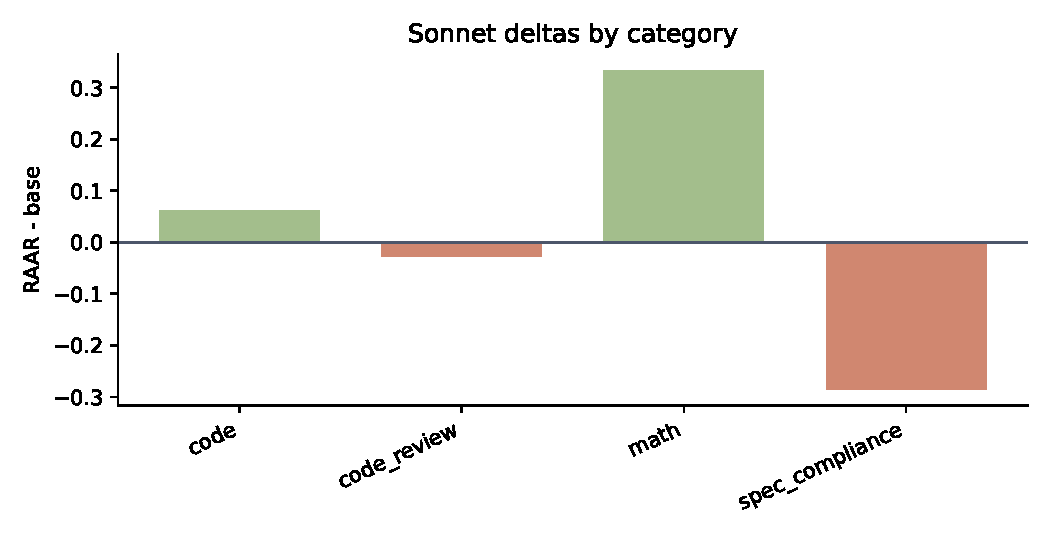
\includegraphics[width=\columnwidth]{fig_domain.pdf}
\caption{Study~2 Sonnet deltas by category. Positive bars indicate
\method{} helps the Sonnet tier on average within that category.}
\label{fig:domain}
\end{figure}

\begin{table}[t]
\caption{Study~2 domain-effectiveness map from numeric checker scores only.
$\Delta$ = \method{} $-$ base within category; omitted cells had no scored
base/RAAR overlap.}
\label{tab:domainmap}
\centering
\scriptsize
\setlength{\tabcolsep}{2pt}
\begin{tabular}{lcccc}
\toprule
category & verif. & Haiku $\Delta$ & Sonnet $\Delta$ & verdict \\
\midrule
code & high & $-0.012$ ($n{=}4$) & $+0.062$ ($n{=}4$) & neutral \\
code review & med. & $+0.083$ ($n{=}1$) & $-0.028$ ($n{=}1$) & mixed \\
math & high & $+0.625$ ($n{=}4$) & $+0.333$ ($n{=}4$) & \shortstack{helps\\strongly} \\
spec compl. & high & $+0.238$ ($n{=}2$) & $-0.286$ ($n{=}2$) & neutral \\
\bottomrule
\end{tabular}
\end{table}

The practical playbook is therefore narrow and actionable. Use \method{}
when the task is verification-shaped --- with the clearest v2 support on
math-like work --- and when the underlying tier still has headroom. Code-review
evidence is tiny-n and mixed, so we do not treat it as strong support. That is
where the detector-generator asymmetry appears most useful. Do not reach for it first on coherence-shaped
prose, as the \emph{explain\_raft} loss and the Study~1 explanation task both
warn. Be skeptical on spec-compliance tasks once the tier is already
capable: effects there are mixed and near zero. And do not replace the
role-separated scaffold with a bare direct answer: the base-direct ablation is
the largest Sonnet-tier drop even though it no longer separates cleanly from
noise.

\subsection{Practical Numbers and Incomplete Cells}
For a usage-based-pricing reader, the headline numbers are straightforward.
One tier down plus \method{} gets surprisingly close on the part of the
distribution that is rich in checkable structure: Sonnet+\method{} closes
about 73\% of the filtered Fable gap on the 5 common primary tasks where
Fable's headroom over Sonnet exceeds 0.05, yet remains 0.137 behind Fable
over all 10 common scored tasks ($p{=}0.127$). The cost is roughly a
ten-call cheaper-tier budget: across all scored runs, the
collected Sonnet+\method{} runs average 10.2 calls, and the Haiku+\method{}
runs 9.9. Two tiers down does not recover: Haiku+\method{} lifts absolute
quality, but its mean gap closure is only 0.304 with a confidence interval
that crosses zero.

Lost cells are part of the result, not bookkeeping noise. The released JSON
contains failed-run no-answer rows for the still-incomplete equal-scaffolding
frontier matrix, and the expanded Fable-base probes add failed no-answer
single-pass rows for \emph{perm\_constraints} and \emph{seq\_runs}. Those
salvaged attempts yielded no scoreable answer and are treated as collection
failures, not as model-quality scores. The artifact is explicit about what
completed, what failed, and what was excluded.

\paragraph*{Does the loop lift the frontier model itself?}
An earlier Fable+\method{} batch was interrupted mid-collection, but the
expanded artifact now contains a narrow completed frontier slice. On six
common scored objective cells spanning five verification-shaped tasks,
raar@fable averages 0.967 versus base@fable at 0.951 on the same five task
means (base@fable is 0.972 over its broader 10-task scored-available macro),
with 0 degraded runs out of 6 compared cells and paired-permutation
$p{=}0.498$ for the +0.015 common-task difference. On this slice the loop
neither lifts nor harms the frontier tier measurably.

\section{Study 1 Mechanism Checks}
\label{sec:analysis}
The transcript-level analyses below remain specific to Study~1, which is the
only study with the full predecessor/successor loop comparison and the
full sanitized role-separated message transcripts needed to diagnose
mechanism.

\subsection{Gate Behavior}
\label{sec:gate-analysis}
Across the 14 objective \method{} runs the gate issued 22 verdicts: 9 PASS,
13 FAIL. Eight of 14 first-round fused answers were refused --- the
adversarial mandate demonstrably does not rubber-stamp. By task: both T1
and both T2 runs passed the first gate; all four T4 runs and two of three
T3a runs drew first-gate refusals; T3b runs were refused twice and passed
once on the first gate. Five runs (36\%) exhausted the $R{=}2$ revision
cap still under verdict FAIL --- and, per Algorithm~\ref{alg:raar}, a
cap-exhausted run returns its final revision \emph{unverified}. In our
data those five unverified finals scored well (a T4 run that left the gate
at FAIL/FAIL scored 12/12; both cap-exhausted T3a runs ended exactly
correct, including the poisoned-rubric run), so in no observed run did the
gate's false-FAIL direction cost correctness rather than compute --- but
this is an empirical observation about 5 runs, not a property the design
guarantees. The converse error matters more: in the two T4 runs with a
residual defect, it was the same constraint both times --- the exact
first-sentence word count. Counting is the one
faculty where detector and generator share the \emph{same} weakness, so the
geometric-suppression argument of Section~\ref{sec:kick} loses its
decorrelation premise; this is the boundary of the method, and we report it
as such.

\subsection{Case Study: a Poisoned Rubric Cannot Derail the Loop}
\label{sec:rubric-case}
The sharpest stress test of \method{} arrived uninvited. In one T3a run
the Stage-1 rubric instance \emph{violated its no-solving instruction}:
its first criterion declared ``the response's final count equals the true
value 397{,}530'' --- a number it had derived itself, incorrectly. The
wrong target was thereby baked into the grading contract that every
downstream verifier inherited, the worst-case failure of rubric
externalization. The gate duly FAILed the (correct) fused answer of
293{,}749 twice. The loop survived anyway: because revision instances are
instructed to \emph{re-verify every flagged defect} rather than obey the
report, the reviser re-derived the count, rejected the rubric's figure,
and the run exhausted its cap still holding 293{,}749 --- scoring 1.0.
Robustness to wrong critiques --- even a wrong \emph{rubric} --- is a
direct consequence of burden-flipping: in \method{}, critiques and
criteria are claims to be checked, never instructions to be applied. The
episode also tempers the Stage-1 design claim: rubric exogeneity is an
instructed tendency, not a guarantee, and the loop's safety rests on the
re-verification discipline beneath it.

\subsection{Case Study: How Self-Refine Destroys a Correct Answer}
\label{sec:selfrefine-case}
The shipped T3a Self-Refine transcripts show the corruption mechanism in
full. A draft entered refinement holding the correct 293{,}749. The
self-critique conceded the answer's format was correct, then applied an
independence heuristic of its own invention --- multiplying the
unconstrained count by $0.9^6$ for the adjacency constraints --- to
declare a ``plausible band'' of roughly 215{,}000--235{,}000, flagged the
correct answer as ``noticeably above that band,'' and ordered the
refinement to ``not trust 293{,}749 --- recompute from scratch.'' The
hand recomputation then slipped, as hand recomputations do; one run's
final answer, 220{,}815, landed \emph{inside the wrong heuristic's band}
--- the model refined its answer toward its own critique's mistaken
expectation. Three independent trajectories produced three different
wrong answers, the instability signature of critique uncorrelated with
truth. The structural diagnosis: the critic shares the generator's context
and commitments, so its objections sample from the same error distribution
as the generation, and iterating that loop performs a random walk around
the answer. \method{}'s verifiers are instead anchored to per-criterion
evidence obligations and mandatory recomputation --- and its revisers are
licensed to reject the critique itself, which is what saved the
poisoned-rubric run above.

\subsection{Cost}
\method{} spends $9$--$12$ base-model calls ($10.5$ mean) against a
single-pass target's 1; stages 2 and 3 parallelize, so the critical path is 5--7
sequential calls. Whether the trade is favorable is a deployment question
that depends on the price ratio between generations at the time of use,
and we make no economic claim. The scientific claim is orthogonal to
price: the measured quality difference is, on these tasks and under these
bounded conditions, partly \emph{recoverable from the base weights} by
structure alone.

\section{Code, Data, and Reproducibility}
\label{sec:reproducibility}
The companion artifact is organized so that each claim can be traced back to
source prompts, raw outputs, scored rows, judge manifests, transcripts where
available, and analysis scripts. Study~1 task prompts and checkers are under
\texttt{bench/tasks/} and \texttt{bench/checkers/}, with scored objective rows
in \texttt{results/all\_objective.scored.json}. Sanitized Study~1
role-separated message transcripts are under
\texttt{results/transcripts/study1\_math\_batch/}; they preserve ordered
user/assistant message content while removing local workflow metadata. Study~2
task prompts are the
\texttt{prompt} fields in \texttt{bench/v2/tasks/*/task.json}; the structural
benchmark validator is \texttt{bench/v2/validate.py}; raw and scored runs are
under \texttt{results/v2/}; and the statistics used in the paper are produced
from \texttt{results/v2/all\_runs.scored.json} by
\texttt{analysis/v2\_stats.py}. The RAAR role prompts, rubric prompt,
verification prompt, fusion prompt, revision prompt, and ablation arms are in
\texttt{harness/lvup.py} and \texttt{harness/lvup\_runner\_v2.js}. Blinded
judged-task prompts, manifests, and verdicts are under
\texttt{results/judging/} and \texttt{results/v2/judging/}.

The intended reproduction path is: run \texttt{bench/v2/validate.py} to check
the benchmark package; run \texttt{analysis/v2\_stats.py} on
\texttt{results/v2/all\_runs.scored.json} to regenerate
\texttt{results/v2/stats.json} and the printed tables; run
\texttt{analysis/v2\_domain\_map.py} for the domain-effectiveness summary;
run \texttt{analysis/v2\_judging/aggregate\_judgments.py} for judged-task
aggregates; and rebuild the PDF from \texttt{paper/main.tex} with the five
included figure PDFs. The paper reports completion-conditional scored means
and separately describes missing/no-answer cells; it does not impute failed
collections as model scores.

\section{Limitations}
\label{sec:limitations}
\textbf{Adversarial audit.} An independent adversarial reviewer (a
separate model family, instructed to break the central claim) raised three
issues we treat as load-bearing. (i)~\emph{Benchmark hardening}: the four v2
code-task checkers originally let candidate code reach the shipped hidden
fixtures, so a fixture-reading cheat submission could score perfectly. No
evaluated model exploited this --- all submissions are genuine solutions, so
the reported scores are unchanged --- and the released artifact ships a hardened-checker
patch that runs candidates in an isolated working directory with the
fixtures inaccessible; the benchmark should be treated as contamination-proof
for reuse only \emph{with} that patch applied. (ii)~\emph{Headline
fragility}: the 0.733 Sonnet gap-closure figure depends on the $>$0.05
tiny-denominator headroom cutoff and ranges over 0.50--0.73 (0.42 pooled);
we now report the full sensitivity. (iii)~\emph{No equal-scaffolding frontier
control}: the headline compares Sonnet+\method{} against \emph{unscaffolded}
Fable, not Fable+\method{}; our partial Fable+\method{} slice (0.967 vs.\
0.951 base on five common tasks, $+0.015$, $p{=}0.498$; base@fable is 0.972
over the broader 10-task scored macro) is consistent with no measurable
frontier lift but does not establish equal-scaffolding parity. The honest
surviving claim is therefore the
narrow one: on a filtered verification-shaped subset, one tier down plus
\method{} recovers roughly half to three-quarters of the gap to unscaffolded
frontier output; the stronger ``approaches the frontier'' reading is not
established by these data.

\textbf{Scale and incompleteness.} Both studies are intentionally small.
Study~1 has 8 tasks and 2--4 runs per objective cell; Study~2 has 15 tasks
overall, but primary objective inference rests on 11 tasks, and judged
comparisons on 1--2 generations per arm. Several Study~2 cells are
explicitly missing as failed no-answer runs: the entire Opus+\method{}
objective batch and two Fable single-pass cells are recorded as failed
no-answer collections; the completed Fable+\method{} batch covers 5 common
objective tasks and 2 judged tasks. The large effects are
informative; small differences are not.

\textbf{Primary-analysis exclusions.} \texttt{constrained\_writing\_16} is
part of the v2 benchmark but excluded from primary analysis because collection
failed and left an unbalanced no-answer partial cell. Some Study~2 figures
therefore show scored-available summaries rather than a perfectly balanced
matrix; the inferential claims always come from the common-task permutation
tests in \texttt{stats.json}.

\textbf{No content-filter attribution.} We do not attribute failed no-answer
rows, missing cells, or RAAR gate refusals to provider content filters or
moderation events. The artifacts do not record such provider-side metadata, so
these rows are treated only as failed/no-answer collection artifacts and not as
evidence about safety filtering.

\textbf{Checker granularity.} v2's near-miss files prove that checkers can
distinguish plausible flawed answers from references, but they are not
semantic calibrations of error severity. Some exact-output transformation tasks
use line- or case-level partial credit, so their numeric partial scores should
be read as deterministic task scores rather than calibrated human utility.

\textbf{Missing and weak ablations.} Study~1 points strongly at the gate,
but Study~2 does not clearly replicate that advantage at Sonnet tier. The
available Sonnet ablations are still thin, partially missing, and mostly
single-run outside the expanded key cells. Approval-exit, no-rubric,
best-of-10, and Self-Refine are therefore useful negative evidence, not
clean component isolations. Fully call-matched, fully completed component
ablations remain future work.

\textbf{Asymmetric scaffolding by construction.} Study~1 asks what is
recoverable from older weights against a successor \emph{as deployed}, so
only the predecessor is scaffolded. Study~2 asks the practical cheaper-tier
question, but the full-ladder equal-scaffolding matrix remains incomplete
even after the added Fable+\method{} cells, so the frontier-loop claim is
limited to a narrow verification-shaped slice.

\textbf{No GPT-5.5 generation arm.} The v2 scored artifact contains
generation rows for Haiku, Sonnet, Opus, and Fable only. GPT-5.5 appears in
the judging artifacts, not in \texttt{all\_runs.scored.json} as generated
answers. A valid GPT-5.5
generator comparison would require a new, same-protocol collection pass with
the same no-tools setting, base/direct and \method{} arms, scoring scripts,
and missing-cell accounting. Until then, GPT-5.5 should be treated as a judge
in this paper, and as a proposed generator extension rather than a generator
result.

\textbf{Task-shape boundaries.} The combined result is not that \method{}
dominates. Study~1's explanation task and Study~2's \emph{explain\_raft}
cell both show a coherence-shaped weakness, while exact counting leaves a
residual gap even in Study~1. Tool grounding would likely change those
boundaries; we exclude tools here to keep the claim purely about call
structure.

\textbf{Judge validity.} Open-ended results still rest on LLM judges. We
mitigated the addressable biases with blind anonymization and position
swaps, and Study~2 simplified the panel after Study~1 showed that the
Claude judges never flipped cross-family majorities. Even so, judged cells
are few, correlated, and only a proxy for expert human evaluation.

\textbf{Inference-setting opacity.} Arms ran at vendor-default settings via
the Claude Code subagent interface; provider-side configuration
(e.g.\ reasoning defaults) is not independently controllable by us. The
comparison is therefore ``deployed default vs.\ deployed default,'' which
matches the practical question but not a parameter-matched laboratory ideal.

\section{Conclusion}
These two studies answer two different deployment questions with the same
loop. Study~1 shows that a direct cross-generation gap can be materially
recovered from older weights alone: on \bench{} v1, \method{} recovers 5 of
the 7 constraint checks that constitute the entire objective gap
(71\%), reaching 0.992 vs.\ 1.000 macro-average with no degraded run
observed in 14. Study~2 broadens the claim from predecessor vs.\ successor
to cheaper tier vs.\ frontier tier: on \bench{} v2, one tier down plus
\method{} closes 0.50--0.73 (threshold-dependent; 0.42 pooled) of the
filtered gap to \emph{unscaffolded} Fable on the verification-shaped tasks
where Sonnet still trails Fable by more than 0.05 under the documented
headroom rule --- not an equal-scaffolding frontier-equivalence result, since
the Fable+\method{} control is incomplete --- but two tiers down does not recover,
and the open-ended coherence gap remains.

The mechanism is not merely more calls, but \emph{differently structured}
inference. Study~1 already showed that best-of-3 changes nothing while
Self-Refine can catastrophically destroy a correct reasoning answer; the v2
direct-answer control sharpens that diagnosis by showing that removing the
role-separated scaffold drops Sonnet from 0.820 to 0.478 (matched-task
$\Delta=-0.341$, $p{=}0.061$). At the same time, Study~2 tempers any
stronger claim: the specific gate advantage that looks salient in Study~1
does not clearly replicate at Sonnet tier, Self-Refine is numerically higher
than full \method{} on the matched Sonnet slice (0.901 vs.\ 0.820) but not
statistically separable at this $n$, and the judged open-ended gap is not
closed even one tier down.

The practical reading is therefore precise rather than universal. If the
task is verification-shaped and the cheaper tier still has headroom,
\method{} can buy back a meaningful share of the gap to unscaffolded
frontier output at roughly a ten-call budget. If the task is coherence-shaped prose, already-near-ceiling
spec compliance, or a two-tier drop, the loop is not enough. The scientific
reading is the same in stricter language: some capabilities measured by a
generation or tier gap are latent in the weaker model and extractable by
orchestration alone, but the recoverable share is sharply bounded by task
shape, model tier, and the quality of the model's own verification.

That boundary is the main product of the paper. The artifact is meant to give
future work concrete handles: complete the equal-scaffolding frontier matrix,
add non-Claude generator families, replace LLM-judged tails with human or
expert panels, and isolate rubric, verifier, fusion, and gate components under
call-matched controls. If those extensions move the boundary, the present
paper should make it clear which part moved and why.

\begin{thebibliography}{40}

\bibitem{snell2024} C.~Snell, J.~Lee, K.~Xu, and A.~Kumar, ``Scaling LLM
test-time compute optimally can be more effective than scaling model
parameters,'' \emph{ICLR}, 2025. arXiv:2408.03314.

\bibitem{brown2024} B.~Brown, J.~Juravsky, R.~Ehrlich, R.~Clark, Q.~V.~Le,
C.~R\'e, and A.~Mirhoseini, ``Large language monkeys: Scaling inference
compute with repeated sampling,'' arXiv:2407.21787, 2024.

\bibitem{cobbe2021} K.~Cobbe \emph{et al.}, ``Training verifiers to solve
math word problems,'' arXiv:2110.14168, 2021.

\bibitem{huang2023} J.~Huang, X.~Chen, S.~Mishra, H.~S.~Zheng, A.~W.~Yu,
X.~Song, and D.~Zhou, ``Large language models cannot self-correct reasoning
yet,'' \emph{ICLR}, 2024. arXiv:2310.01798.

\bibitem{stechly2024} K.~Stechly, K.~Valmeekam, and S.~Kambhampati, ``On the
self-verification limitations of large language models on reasoning and
planning tasks,'' arXiv:2402.08115, 2024.

\bibitem{liang2023} T.~Liang \emph{et al.}, ``Encouraging divergent thinking
in large language models through multi-agent debate,'' \emph{EMNLP}, 2024.
arXiv:2305.19118.

\bibitem{panickssery2024} A.~Panickssery, S.~Bowman, and S.~Feng, ``LLM
evaluators recognize and favor their own generations,'' \emph{NeurIPS},
2024. arXiv:2404.13076.

\bibitem{wataoka2024} K.~Wataoka, T.~Takahashi, and R.~Ri,
``Self-preference bias in LLM-as-a-judge,'' arXiv:2410.21819, 2024.

\bibitem{song2024} Y.~Song, H.~Zhang, C.~Eisenach, S.~Kakade, D.~Foster, and
U.~Ghai, ``Mind the gap: Examining the self-improvement capabilities of
large language models,'' arXiv:2412.02674, 2024.

\bibitem{stroebl2024} B.~Stroebl, S.~Kapoor, and A.~Narayanan, ``Inference
scaling flaws: The limits of LLM resampling with imperfect verifiers,''
arXiv:2411.17501, 2024.

\bibitem{tick2024} J.~Cook \emph{et al.}, ``TICKing all the boxes:
Generated checklists improve LLM evaluation and generation,''
arXiv:2410.03608, 2024.

\bibitem{rar2025} A.~Gunjal \emph{et al.}, ``Rubrics as rewards: Reinforcement
learning beyond verifiable domains,'' arXiv:2507.17746, 2025.

\bibitem{liu2025} R.~Liu \emph{et al.}, ``Can 1B LLM surpass 405B LLM?
Rethinking compute-optimal test-time scaling,'' arXiv:2502.06703, 2025.

\bibitem{s1_2025} N.~Muennighoff \emph{et al.}, ``s1: Simple test-time
scaling,'' arXiv:2501.19393, 2025.

\bibitem{setlur2025} A.~Setlur, N.~Rajaraman, S.~Levine, and A.~Kumar,
``Scaling test-time compute without verification or RL is suboptimal,''
arXiv:2502.12118, 2025.

\bibitem{gema2025} A.~P.~Gema \emph{et al.}, ``Inverse scaling in test-time
compute,'' \emph{TMLR}, 2025. arXiv:2507.14417.

\bibitem{madaan2023} A.~Madaan \emph{et al.}, ``Self-Refine: Iterative
refinement with self-feedback,'' \emph{NeurIPS}, 2023. arXiv:2303.17651.

\bibitem{shinn2023} N.~Shinn, F.~Cassano, E.~Berman, A.~Gopinath,
K.~Narasimhan, and S.~Yao, ``Reflexion: Language agents with verbal
reinforcement learning,'' \emph{NeurIPS}, 2023. arXiv:2303.11366.

\bibitem{li2023gv} X.~L.~Li, V.~Shrivastava, S.~Li, T.~Hashimoto, and
P.~Liang, ``Benchmarking and improving generator-validator consistency of
language models,'' \emph{ICLR}, 2024. arXiv:2310.01846.

\bibitem{huang2024sharpening} A.~Huang \emph{et al.}, ``Self-improvement in
language models: The sharpening mechanism,'' arXiv:2412.01951, 2024.

\bibitem{wang2022} X.~Wang \emph{et al.}, ``Self-consistency improves chain
of thought reasoning in language models,'' \emph{ICLR}, 2023.
arXiv:2203.11171.

\bibitem{jiang2023} D.~Jiang, X.~Ren, and B.~Y.~Lin, ``LLM-Blender:
Ensembling large language models with pairwise ranking and generative
fusion,'' \emph{ACL}, 2023. arXiv:2306.02561.

\bibitem{wang2024moa} J.~Wang \emph{et al.}, ``Mixture-of-Agents enhances
large language model capabilities,'' \emph{ICLR}, 2025. arXiv:2406.04692.

\bibitem{selfmoa2025} W.~Li \emph{et al.}, ``Rethinking
Mixture-of-Agents: Is mixing different large language models beneficial?''
arXiv:2502.00674, 2025.

\bibitem{du2023} Y.~Du, S.~Li, A.~Torralba, J.~B.~Tenenbaum, and
I.~Mordatch, ``Improving factuality and reasoning in language models through
multiagent debate,'' \emph{ICML}, 2024. arXiv:2305.14325.

\bibitem{smit2024} A.~P.~Smit \emph{et al.}, ``Should we be going MAD? A
look at multi-agent debate strategies for LLMs,'' \emph{ICML}, 2024.
arXiv:2311.17371.

\bibitem{checkeval2024} Y.~Lee \emph{et al.}, ``CheckEval: A reliable
LLM-as-a-judge framework for evaluating text generation using checklists,''
\emph{EMNLP}, 2025. arXiv:2403.18771.

\bibitem{ruscarl2025} Y.~Zhou \emph{et al.}, ``Breaking the exploration
bottleneck: Rubric-scaffolded reinforcement learning for general LLM
reasoning,'' arXiv:2508.16949, 2025.

\bibitem{wangfair2023} P.~Wang \emph{et al.}, ``Large language models are
not fair evaluators,'' \emph{ACL}, 2024. arXiv:2305.17926.

\bibitem{zheng2023} L.~Zheng \emph{et al.}, ``Judging LLM-as-a-judge with
MT-Bench and Chatbot Arena,'' \emph{NeurIPS Datasets and Benchmarks}, 2023.
arXiv:2306.05685.

\bibitem{yang2024sweagent} J.~Yang \emph{et al.}, ``SWE-agent:
Agent-computer interfaces enable automated software engineering,''
\emph{NeurIPS}, 2024. arXiv:2405.15793.

\bibitem{xia2024agentless} C.~S.~Xia, Y.~Deng, S.~Dunn, and L.~Zhang,
``Agentless: Demystifying LLM-based software engineering agents,''
arXiv:2407.01489, 2024.

\bibitem{saadfalcon2025} J.~Saad-Falcon \emph{et al.}, ``Shrinking the
generation-verification gap with weak verifiers,'' \emph{NeurIPS}, 2025.
arXiv:2506.18203.

\bibitem{weiblog2025} J.~Wei, ``Asymmetry of verification and verifier's
law,'' Blog post, Jul.\ 2025. [Online]. Available:
\url{https://www.jasonwei.net/blog/asymmetry-of-verification-and-verifiers-law}

\end{thebibliography}

\end{document}
